\section{GeoSN Query Process System}

We overview the literature on GeoSN query processing systems in industry and academia. In what follows, we examine the API exposed by commercial online services, as well as the algorithm and data structure reported in academic projects.

\subsection{Commercial Products}
\subsubsection{Foursquare}
Foursquare’s Radar return the friends who are currently in the vicinity of a user. Foursqaure also expose their API for developers of LBS. The Foursquare API provides methods for accessing a resource such as a venue, tip, or user. In spirit with the RESTful model\cite{restful}, each resource is associated with a URL. For example, information about Clinton Street Baking Co can be found as follows (assuming credentials for such information is verified cryptographically beforehand):

\begin{verbatim}
	https://api.foursquare.com/v2/venues/40a55d80f964a52020f31ee3
\end{verbatim}

Given a resource, you can then drill into a particular aspect, for example

\begin{verbatim}
	https://api.foursquare.com/v2/venues/40a55d80f964a52020f31ee3/tips
\end{verbatim}

Each returned tip will have its own ID, which corresponds to its own resource URL, for example

\begin{verbatim}
	https://api.foursquare.com/v2/tips/49f083e770c603bbe81f8eb4
\end{verbatim}

Foursquare does not expose user's GPS location via its API, and only allows access to venue information (in the \texttt{venuehistory} and \texttt{checkins} aspects of user API). Foursquare also reveals the social network between users via the \texttt{friends} property of any users, which developers can use to get list of friends as follows:

\begin{verbatim}
	https://api.foursquare.com/v2/users/USER_ID/friends
\end{verbatim}

Foursquare does not report how they manage their social network database. However, they use MongoDB for the storage of venues and check-ins\cite{4qrmongo}. The original Foursquare application relied on a single relational database. With this relational architecture, foursquare could not simply and easily scale to many nodes required for a high traffic application. As the company experienced rapid growth, it split the data to two nodes: one for checkins (the biggest data set) and one for everything else. Yet it was clear that check-ins would grow beyond what a single machine could handle, and that a long-term, scalable solution to Foursquare's growth was needed. Foursquare benefits from MongoDB’s support for geospatial indexing, allowing it to easily query for location-based data. 

MongoDB's document model, with independent JSON-like objects, maps well to object-oriented programming, in contrast with the schema-enforced table structures of relational databases. MongoDB allows foursquare to dramatically simplify its data model. For instance, rather than storing tags ('has wifi", "great for dates", "hotspot", etc.) in a separate table and relying on mapping tables and costly JOINs, in MongoDB tags are embedded directly into the document representing a venue. This is both more efficient at run-time, and easier for engineers to understand and manipulate.

\subsubsection{Facebook}
Facebook's Graph API is the primary way for developers to get data in and out of Facebook's platform. Aside from social graph, developers can obtain user's location via \texttt{place} API as follows.

\begin{verbatim}
/* make the API call */
FB.api(
    "/{place-id}",
    function (response) {
      if (response && !response.error) {
        /* handle the result */
      }
    }
);
\end{verbatim}

Each place has a field called \texttt{overall\_rating}, which is the overall rating of Place, on a 5-star scale.

\subsubsection{ArcGIS}
ArcGIS\cite{arcgis} exposes a variety of functionalities to developers, including location services (directions/guidance, geo-trigger\footnote{Geo-trigger notifies a user when friends enter a certain range.}), mapping, and imagery. They claim that their data can be accessed via a RESTful API, but do not disclose details of how their data is managed. It is also unclear whether they have social networking functions in their system based on public information.

\subsection{Academic Efforts}
There has been few literature on GeoSN query processing\cite{amir2007buddy,yiu2010efficient,khoshgozaran2009private,scellato2010distance}. These works did not focus on important data management issues, which potentially undermine their practicality. More specifically, they tie the algorithms with specific data representations and indices, which may incurr significant overhead in large GeoSNs, because data representation scheme greatly affects the performance of any algorithm. Also, all of them assume that all the data are owned by a single entity, and can be handles by a single machine. Their specific problems are as follows:
\begin{itemize}
	\item\cite{khoshgozaran2009private} uses an adjacency matrix for keeping info about the social graph, which may incur prohibitive storage overhead. 
	\item\cite{amir2007buddy,scellato2010distance} make use of hybrid indices of both social and spatial data, which may suffer from enormous maintenance costs due to high check-in rates. 
	\item\cite{yiu2010efficient,scellato2010distance} do not specify how the social graph is stored. 
\end{itemize}

\subsection{A General Framework for Geo-Social Query Processing\cite{armenatzoglou2013general}}
A general framework for processing GeoSN queries is proposed in \cite{armenatzoglou2013general}.
The proposed architecture consists of three modules, depicted in Figure\ref{fig:gen-arch}: a social module (SM), a geographical module (GM), and a query processing module (QM). 
The SM stores only the social graph (e.g., friendship relations), and the GM keeps only geographical information (e.g., check-ins, venues, ratings). The QM is responsible for receiving GeoSN queries from users, executing them, and returning the results. The users do not communicate directly with the SM and GM. The SM, GM and QM can either be three separate servers, three separate clouds, or a single system (server or cloud). However, the tasks of the three modules are segregated.

\begin{figure}[hbt]
  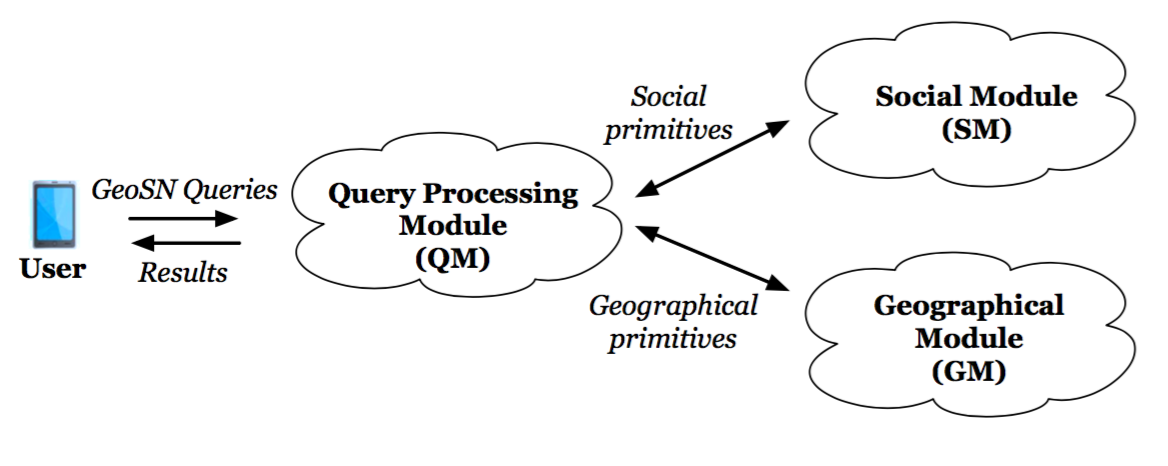
\includegraphics[width=\linewidth]{figs/gen-arch.png}
  \caption{The proposed architecture\cite{armenatzoglou2013general}}\label{fig:gen-arch}
\end{figure}

The SM and GM interact only with the QM using well-defined social and geographical primitive queries. 
The SM and GM only execute their corresponding primitives on their stored data, and the primitives are given by QM based on the algorithms used to process the queries. 
The QM eventually assembles the final results by combining the outputs of the primitives, optionally exploiting auxiliary indices maintained locally.

The segregation of SM and GM allows their administration by different entities, e.g., the SM (GM) can be maintained by a company with expertise in social networking (resp. location-based services). 

For instance, in UK and Japan, Facebook Places [3] cooperates with Factual [4], which provides infrastructure for location- based services. Glancee [12], a location-based service app, uses Facebook’s social graph to connect nearby users. Another example is the cooperation of pure commercial social networks, e.g., Twitter or Facebook, and GeoSNs like Foursquare. A user who has both a Twitter or Facebook and a Foursquare account can post his Foursquare check-in at Twitter or Facebook [15]. Thus, if Facebook or Twitter needs the geographical information of users’ check-ins to execute a GeoSN query, it obtains it from Foursquare. The separation of QM enables third-party companies that do not own any social or geographical data to implement GeoSN queries by solely interacting with the APIs of SM and GM (e.g., Agora [1]).

In addition, separating the functionality of SM and GM renders the management of social and geographical data more flexible, because the frequent check-in updates do not burden the relatively static social structures. 

For example, due to an unexpected high rate of check-ins recently, Foursquare’s system had a very long down- time. The problem was caused because their data are spread across multiple balanced database shards. When a shard is overused, a new one is added, followed by rebalancing. The rebalancing of the entire database caused the crash. In a segregated system, such a crash in GM would not affect SM.

First, our architecture can readily integrate modifications (e.g., a new, more efficient structure) in the implementation of SM without modifying GM, and vice versa. 
Second, novel GeoSN query types and algorithms can be devised, either by using a different combination of existing primitives or by implementing new ones, without the need of altering the SM and GM infrastructures. 
Last, social (geographical) data can be used independently for pure social (resp. geographical) queries, potentially through the same primitive operations utilized by GeoSN queries. 
As a result, a “traditional” social network can adopt our architecture without extra effort.

\begin{comment}
Primitive Queries
Here we introduce the primitive social and geographical queries that are used as fundamental components in our GeoSN algorithms (presented in Section 4). These operations are supported by all typ- ical graph and spatial data structures, and can be easily integrated with any SM and GM implementation.
We make use of the following social primitives:
• GetFriends(u): Given a user u, return u’s friends.
• AreFriends(ui,uj): Given two users ui, uj, return true if ui, uj are friends, and false otherwise.
We also utilize the geographical primitives below. Note that ev- ery location is regarded as a (x,y) pair of coordinates in some fixed Cartesian plane. When we refer to a user’s location, we mean the (x,y) coordinates associated with his/her current (i.e., lastly posted) check-in. We assume Euclidean space, but the gen- eral framework and query processing techniques also apply for road networks (the GM should simply integrate an indexing scheme that supports the primitives according to the network distance, e.g., [35]).
• GetUserLocation(u): Given u, return u’s location.
• RangeUsers(q, r): Given a query point q and a real number r, return the users within distance r from q, along with their locations.
• NearestUsers(q,k): Given a query point q and an integer k, return the k users nearest to q in ascending distance, along with their locations.
Observe that RangeUsers and NearestUsers return also the lo- cation of each user in the result. This could be very useful for the algorithms at QM that employ these primitives, while it does not affect the computational and space complexity of the result.
All the above primitives can be easily supported by the API of SM and GM. For instance, GetFriends is readily implemented in the API of Facebook, whereas the API of Foursquare offers GetUserLocation. We do not exclude the existence of additional primitives. Nevertheless, any primitive must be treated as an atomic operation. To the best of our knowledge, operations that maintain state for future primitive invocations (e.g., an incremental version of a nearest neighbor query that extracts the next best result upon a new query) are not supported by any commercial GeoSN. The main reason is that maintaining state (e.g., via priority queues) for a large number of simultaneous queries is prohibitively expensive.
The efficiency of the primitives depends on the underlying stor- age scheme employed by SM and GM. For instance, representing the social graph by adjacency lists is preferable for GetFriends (the output simply consists of the users in the list of u), whereas adjacency matrices are faster for AreFriends (the output is true if the bit at cell (i,j) of the matrix is 1). Similarly, although all common spatial indices support RangeUsers and NearestUsers, they feature differences in performance.
Unfortunately, there is no unanimously accepted social or spatial storage implementation. To elaborate, Facebook uses adjacency lists stored in Memcached [16], a distributed memory caching sys- tem, whereas Foursquare uses MongoDB [17], a document-oriented database. Moreover, Twitter employs the R*-Tree spatial index [20], whereas Foursquare adopts the grid-based geohashes of Mon- goDB [11]. Similarly, academic research has utilized a wide vari- ety of approaches; [27] uses adjacency lists stored in Neo4j [18] (a graph database), [31] employs an adjacency matrix, whereas [26] utilizes relational tables for storing the friendship relations; more- over, [23] indexes check-ins with a grid, [21] applies a Quad tree, while [31] exploits the R*-Tree. We stress that every GeoSN algo- rithm should be tailored to a specific SM and GM instantiation, se- lecting the combination of primitives that leads to maximum query efficiency. In the next section, we explain that a variety of GeoSN algorithms can be implemented using the described primitives.
\end{comment}